\chapter{Anwendungen}
\label{Anwendungen}

In diesem Kapitel wird beschrieben, wie Dijkstra- und Bellman-Algorithmen in realen Anwendungen angewendet werden können.


\section{GIS(Geoinformationssystem)}
\label{GIS(Geoinformationssystem)}
\subsection{Definition}


nach Vaibhavi Patel und Prof.Chitra Baggar „Ein geografisches Informationssystem (GIS) ist ein computergestütztes Werkzeug. Mit diesen Werkzeugen können wir räumliche Informationen erstellen, manipulieren, analysieren, speichern und anzeigen. Räumliche Informationen sind Informationen über Objekte, die sich auf der Erde befinden, wie z. B. Städte, Eisenbahnstrecken, Flüsse usw“\footnote{GIS Definition \cite{Vaibhavi2014}}. 

\subsection{Geoinformationssystem mit Dijkstra-Algorithmus}
Obwohl dieser Dijkstra-Algorithmus sehr effektiv zu sein scheint, kann es im Grunde genommen sehr lange dauern, die Route vom Start bis zum Ende weiterzuleiten, wobei eine große Menge an Informationen verwendet wird, wie in der Abbildung 4.1 zu sehen ist, was überhaupt nicht angemessen ist, so dass eine Alternative entwickelt werden muss, um die Zeit zu verkürzen\cite{HamidAli2020}.

\begin{figure}[H]
	\centering
	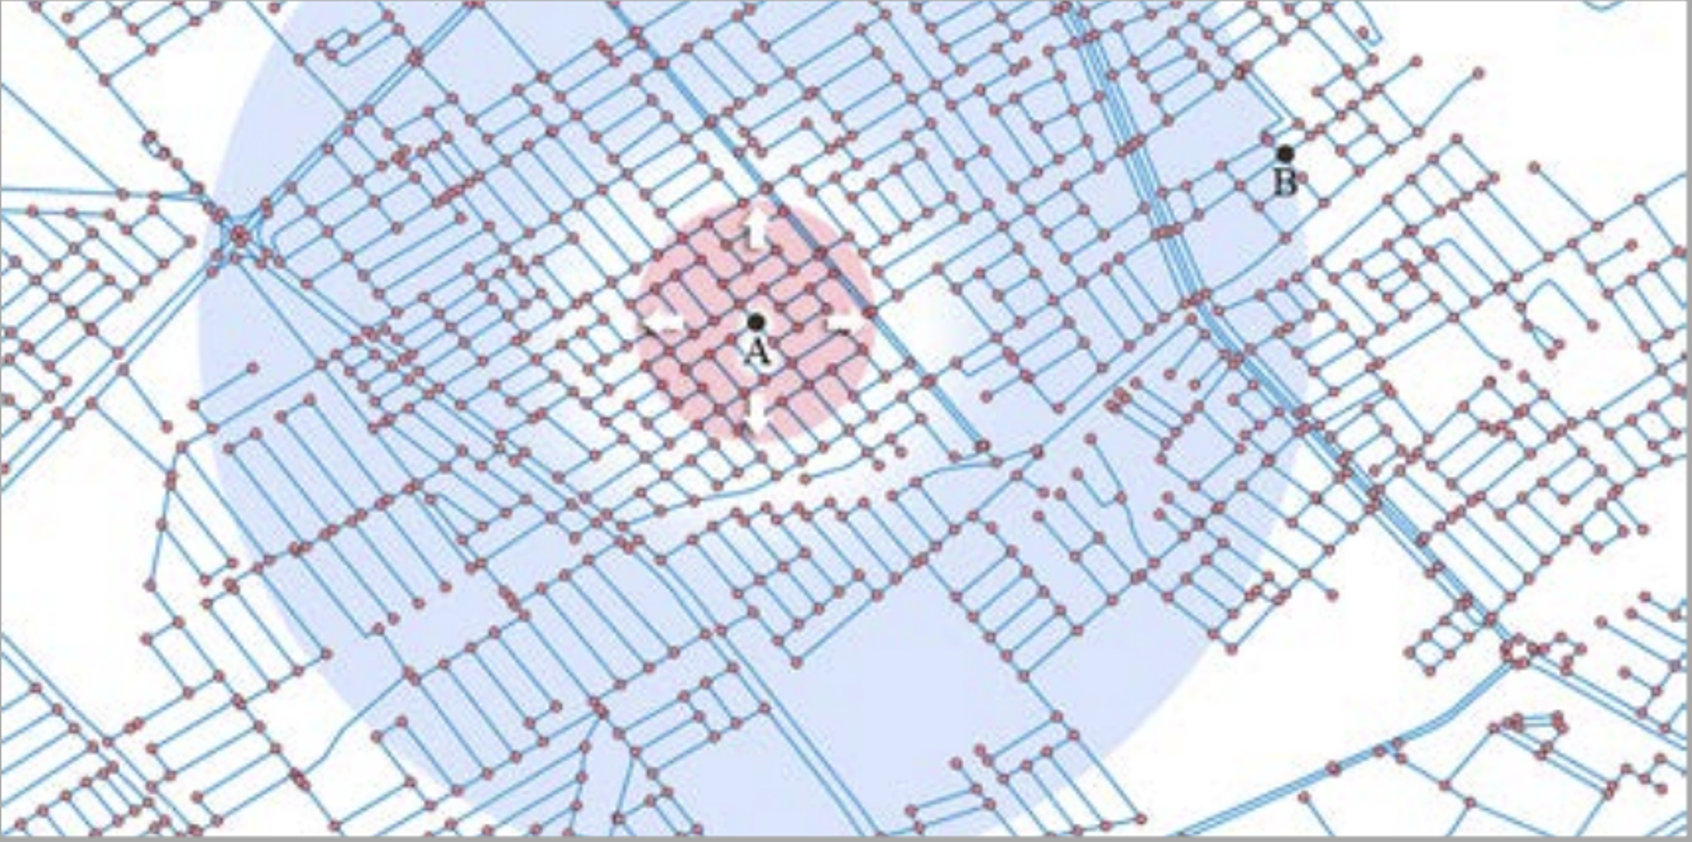
\includegraphics[width=0.7\textwidth]{images/GIS_red.PNG}
	\caption{\label{fig:GIS_red}Dijkstra's Fortschritt\cite{HamidAli2020}.}
\end{figure}

So haben die Autoren des Artikels\footnote{GIS Beispiel \cite{HamidAli2020}}  ihr Experiment wie folgt beschrieben:
\newline
\newline
 „Der rote Kreis stellt den Verlauf des Dijkstra-Algorithmus dar, während der blaue Kreis die tatsächlichen Knoten und Linien des Graphen anzeigt, die der Algorithmus verarbeiten muss, bevor er die korrekte Wurzel von A nach B berechnen kann. Der verbesserte Algorithmus kann den Suchbereich erheblich verkleinern, wie in Abbildung 4.2 dargestellt. Dies ist nur ein Bruchteil des Bereichs in der vorherigen Abbildung. Er ermöglicht wesentlich schnellere Berechnungen und verkürzt damit die Zeit, die der Routing-Prozess benötigt, um einen gültigen Pfad zu finden. Die Verbesserungsmethode besteht im Wesentlichen darin, einen temporären Datensatz zu erstellen, bevor der Dijkstra-Algorithmus selbst gestartet wird, und diesen so zu behandeln, als wäre er der Graph, mit dem der Algorithmus arbeiten muss. Dieser Datensatz wird erstellt, nachdem die Start- und Endknoten erfasst wurden. Mit den Koordinaten der Start- und Endknoten kann der Datensatz aus den Hauptdaten ausgeschlossen werden, indem nur die Knoten ausgewählt werden, die sich innerhalb des von den beiden Knoten gebildeten Quadrats befinden“.

\begin{figure}[H]
	\centering
	\includegraphics[width=0.7\textwidth]{images/GIS_blue.PNG}
	\caption{\label{fig:GIS_red}Verbesserter Suchbereich\cite{HamidAli2020}.}
\end{figure}

\section{Mobile Roboter mit verbessertem Dijkstra-Algorithmus}
\label{Mobile Roboter mit verbessertem Dijkstra-Algorithmus}
\subsection{traditioneller Dijkstra vs verbesserter Dijkstra }

Die Autoren des Artikels\footnote{Vergleich zwischen Standard und verbessert Dijkstra \cite{Karur2021}} haben zitiert dass:
„Der traditionelle Dijkstra-Algorithmus beruht auf einer gierigen Strategie zur Pfadplanung. Er wird verwendet, um den kürzesten Weg in einem Graphen zu finden. Er befasst sich mit der Lösung des kürzesten Weges, ohne sich formal um die Pragmatik der Lösung zu kümmern.
\newline
\newline
 Der modifizierte Dijkstra-Algorithmus zielt darauf ab, alle Knoten mit gleichem Abstand zum Ausgangsknoten als Zwischenknoten zu reservieren, und sucht dann von allen Zwischenknoten aus weiter, bis er erfolgreich zum Zielknoten durchläuft, siehe Abbildung 4.3. Durch Iteration werden alle möglichen kürzesten Wege gefunden und können dann ausgewertet werden“.

\begin{figure}[H]
	\centering
	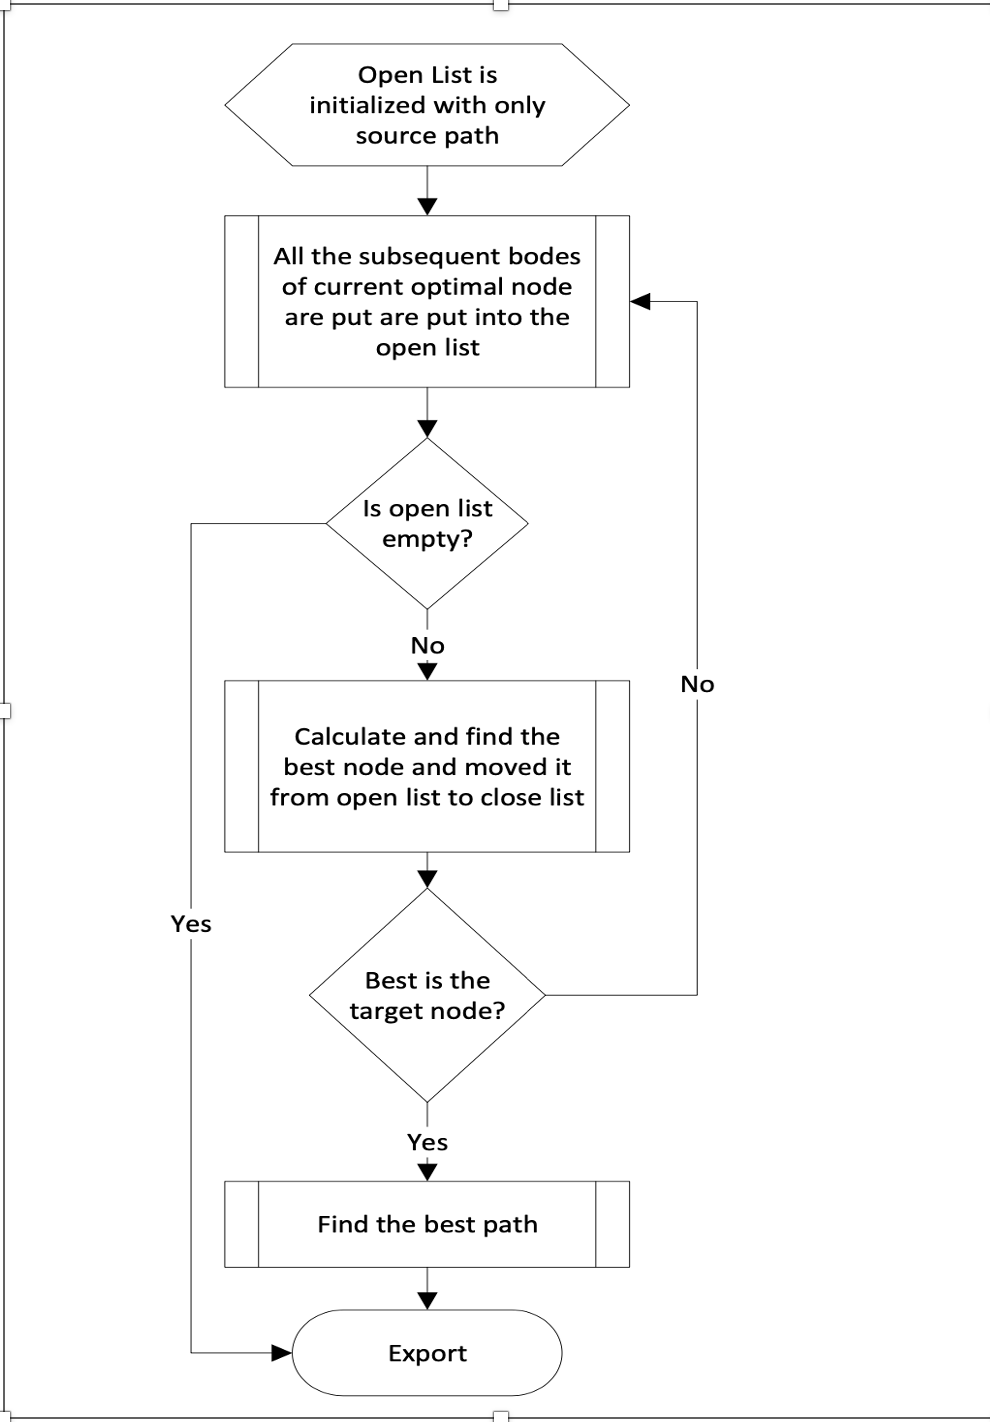
\includegraphics[width=0.7\textwidth]{images/Activity_robot.PNG}
	\caption{\label{fig:Robot}Flussdiagramm des verbesserten Dijkstra für die Pfadplanung\cite{Karur2021}.}
\end{figure}

\subsection{Verbesserter Dijkstra }
Die Autoren des Artikels\footnote{ verbesserter Dijkstra für Mobile Roboter \cite{Karur2021}} haben der verbesserte Dijkstra-Algorithmus so beschrieben:
„Der Dijkstra-Algorithmus kann außer den bereits durchlaufenen Knoten keine Daten speichern. Um diesen Nachteil zu überwinden, wird ein Speicherschema eingeführt, das ein mehrschichtiges Wörterbuch implementiert, das aus zwei Wörterbüchern und einer Liste von Datenstrukturen besteht, die in hierarchischer Reihenfolge organisiert sind. Das erste Wörterbuch bildet jeden einzelnen Knoten auf seine Nachbarknoten ab. Das zweite Wörterbuch speichert die Pfadinformationen jedes benachbarten Pfades.
\newline
\newline

Ein mehrschichtiges Wörterbuch bietet eine umfassende Datenstruktur für den Dijkstra-Algorithmus in einer Innenraumanwendung, bei der die Koordinaten des globalen Navigationssatellitensystems und die Kompassorientierung nicht zuverlässig sind. Die Pfadinformationen in der Datenstruktur helfen dabei, den Grad des Drehwinkels zu bestimmen, den der Roboter an jedem Knoten oder jeder Kreuzung ausführen muss. Der vorgeschlagene Algorithmus liefert den kürzesten Pfad in Bezug auf die Länge und gleichzeitig den navigierbarsten Pfad in Bezug auf den niedrigsten erforderlichen Gesamtdrehwinkel in Grad, der mit dem traditionellen Dijkstra-Algorithmus nicht berechnet werden kann“.

\section{Autonome Navigation}
\label{Autonome Navigation}

Pfadsuchalgorithmen werden ebenfalls im Bereich des Autonomen Fahrens\index{Autonomes Fahren}, oder auch im Bereich der unbemannten Flugfahrzeuge verwendet
um sichere\index{sicher}, effiziente\index{effizient}, kollisionsfreie und kostengünstige Wege von Start zum Ziel zu führen. Die Wahl des richtigen Pfadsuchalgorithmen
ist sehr wichtig, denn es hängt unter anderem die Geometrie des Fahrzeugs von dieser Wahl ab.
Mit der zunehmenden Verbreitung von autonomen Fahrzeugen, die immer mehr Weg- findung und planung erfordert, ist das Thema dieses Papers 
zu einem neuen Schwerpunkt im Bereich der autonomen Steuerung geworden.
Da mobile Roboter\index{Roboter} in vielen Anwendungen eingesetzt werden, haben Forscher Methoden entwickelt, um die 
Anforderungen an mobile Roboter effektiv erfüllen zu können und einige Herausforderungen für die Umsetzung einer vollständig oder
teilweise autonomen Navigation in unübersichtlichen Umgebung zu bewältigen.\cite{Karur:21}

Die Leistung und Komplexität\index{Komplexität} des verwendeten Algorithmus hängt auch vom Anwendungsfall ab. \cite{Karur:21}\\
Somit gibt es nicht \emph{den perfekten Pfadsuchalgorithmus für Autonomes Fahren}, aber es finden viele verschiedene Algorithmen eine 
Anwendung in der autonomen Navigation.